\documentclass{beamer}


\usepackage[utf8]{inputenc}
\usepackage{amsmath}
\usepackage{amsfonts}
\usepackage{amssymb}
\usepackage{graphicx}
\usepackage{ragged2e}  % `\justifying` text
\usepackage{booktabs}  % Tables
\usepackage{tabularx}
\usepackage{tikz}      % Diagrams
\usetikzlibrary{calc, shapes, backgrounds}
\usepackage{amsmath}
\usepackage{amssymb}
\usepackage{dsfont}
\usepackage{url}       % `\url
\usepackage{listings}  % Code listings
\usepackage[T1]{fontenc}


\usepackage{theme/beamerthemehbrs}

\author[]{Abhishek Padalkar}

\title{Dynamic Motion Primitives}
\subtitle{Research and Development Project}
\institute[HBRS]{Hochschule Bonn-Rhein-Sieg}
\date{\today}
\subject{Test beamer}

% \thirdpartylogo{path/to/your/image}


\begin{document}
	{
	\begin{frame}
	\titlepage
	\end{frame}
	}
	
	\begin{frame}{Motivation}
		\begin{itemize}
			\item Humans \textbf{learn} variety of motions and use them in similar situations. 
			\item Human motions consist of motion primitives. 
			\item Concept of motion primitives can be adopted for robots. 
			\item Learned motion primitives can be combined to do complex task. 
			\item Several approaches are available for learning motion primitives.
		\end{itemize}
	\end{frame}
	
	
	\begin{frame}{Advantages of DMP}
		\begin{itemize}
			\item It is a model free learning approach.
			\item Any arbitrary trajectory can be learned in end-effector space as well as in joint space.
			\item Here learning is linear regression, so it does not need large dataset.
			One trajectory is sufficient ideally.
			\item Trajectories can be scaled in space as well as in time.
			\item Trajectory evolves as robot actually moves along the trajectory. Hence on-line modifications in the trajectory are possible.

		\end{itemize}
	\end{frame}

	\begin{frame}{Formulation of DMP}
		\begin{equation}\label{DMP_1}
		\tau\dot{z} = \alpha_{z}(\beta_{z}(g - y) - z) + f(x)
		\end{equation}
		\begin{equation}\label{DMP_2}
		\tau \dot{y} = z
		\end{equation}
		\begin{equation}\label{forcing_term}
		f(x) = \frac{\sum_{i=1}^{N}\psi_{i}(x)w_{i}}{\sum_{i=1}^{N}\psi_{i}(x)}x(g - y_{0})
		\end{equation}
		where,
		\begin{equation}\label{psi}
		\psi_{i} = \exp(-{\frac{1}{2\sigma_{i}^{2}}(x - c_{i})^{2}})
		\end{equation}
		and,
		\begin{equation}\label{canonical}
		\tau \dot{x} = -\alpha_{x}x
		\end{equation}
		
		[$y, \dot{y}, \ddot{y}$] = kinematic state  \\
		$g$ = goal value \\
		$y_{0}$ = initial value
	\end{frame}
	
	
	\begin{frame}
		\begin{itemize}
			\item Second order differential equation representing mass spring damped system. 
			\item Non-linear term \textit{f(x)} modifies the acceleration and characterizes the motion. 
		\end{itemize}
	\end{frame}

	\begin{frame}{Working of DMP}
		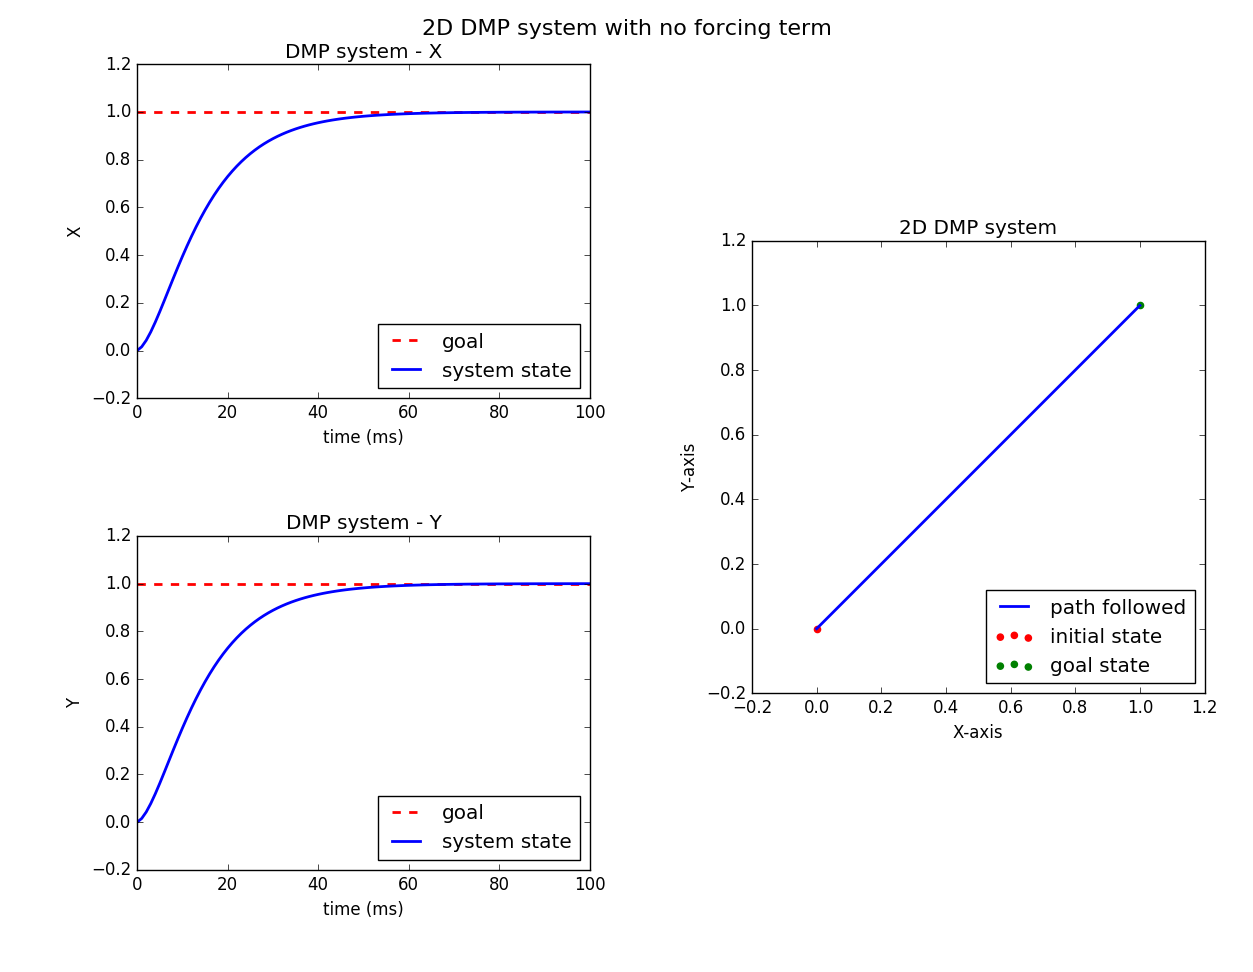
\includegraphics[width=\textwidth]{images/dmp_no_f}
	\end{frame}
	\begin{frame}
		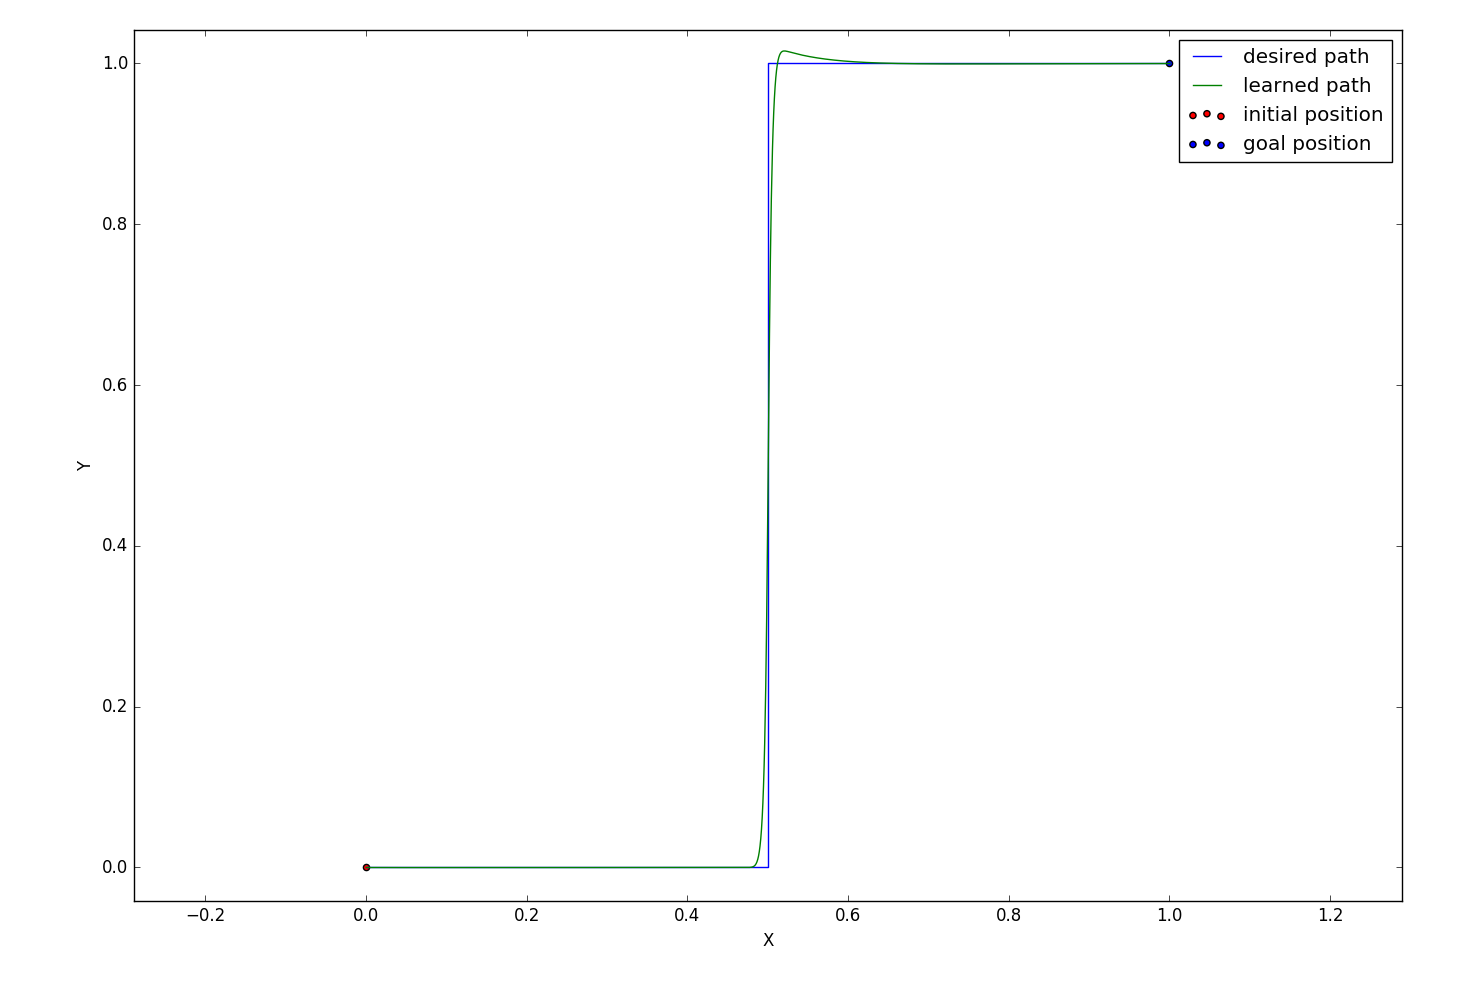
\includegraphics[width=\textwidth]{images/step_f}
	\end{frame}
	\begin{frame}
		\begin{figure}
			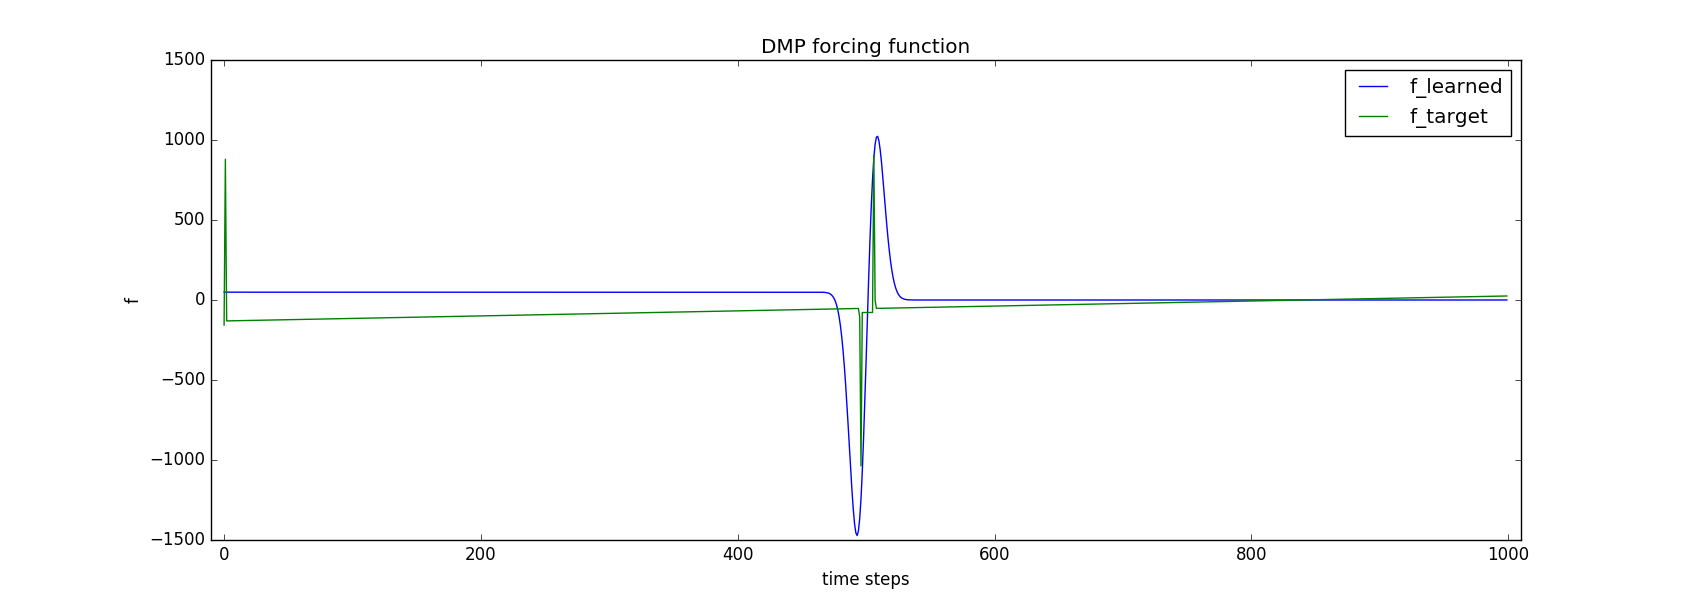
\includegraphics[scale=0.23]{images/f_x}
			\caption{Forcing term - X}
		\end{figure}

		\begin{figure}
			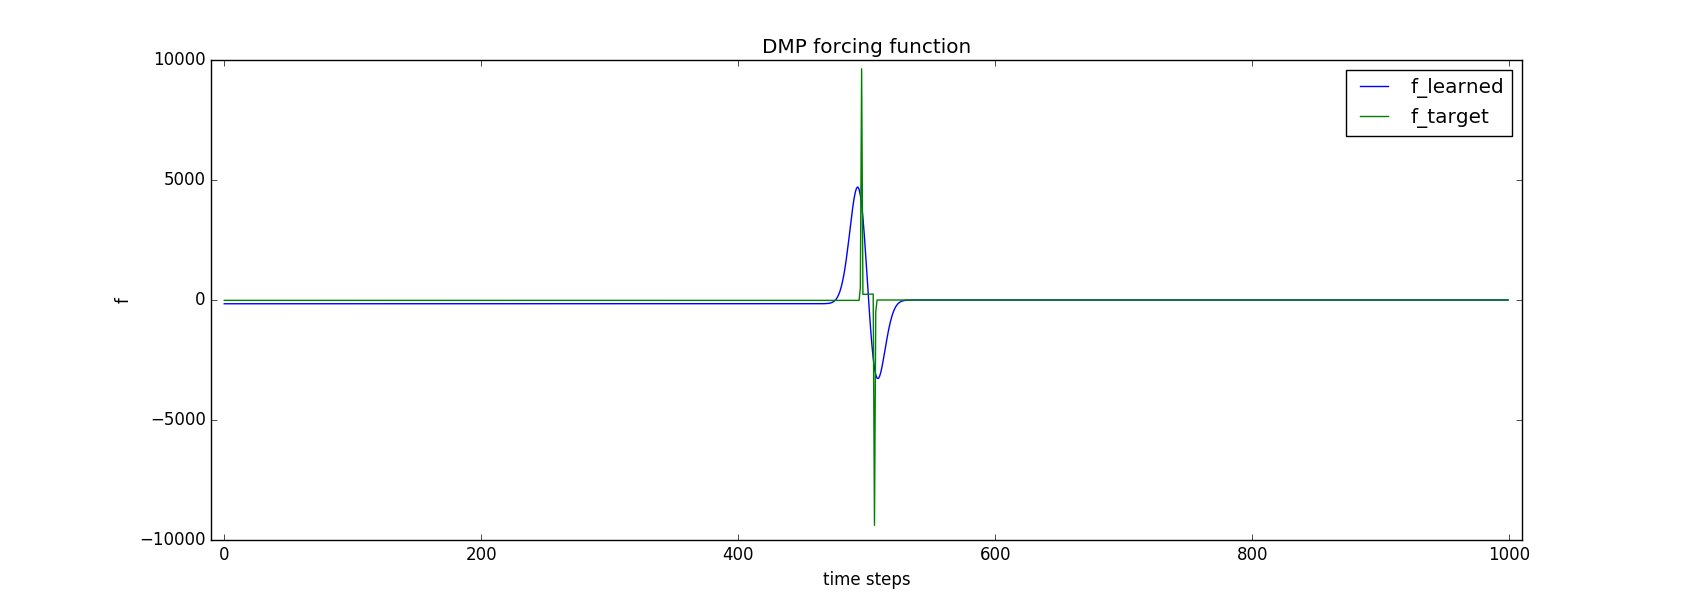
\includegraphics[scale=0.23]{images/f_y}
			\caption{Forcing term - Y}
		\end{figure}

	\end{frame}
	
	\begin{frame}{Analysis of the effects of the parameters used in DMP}
		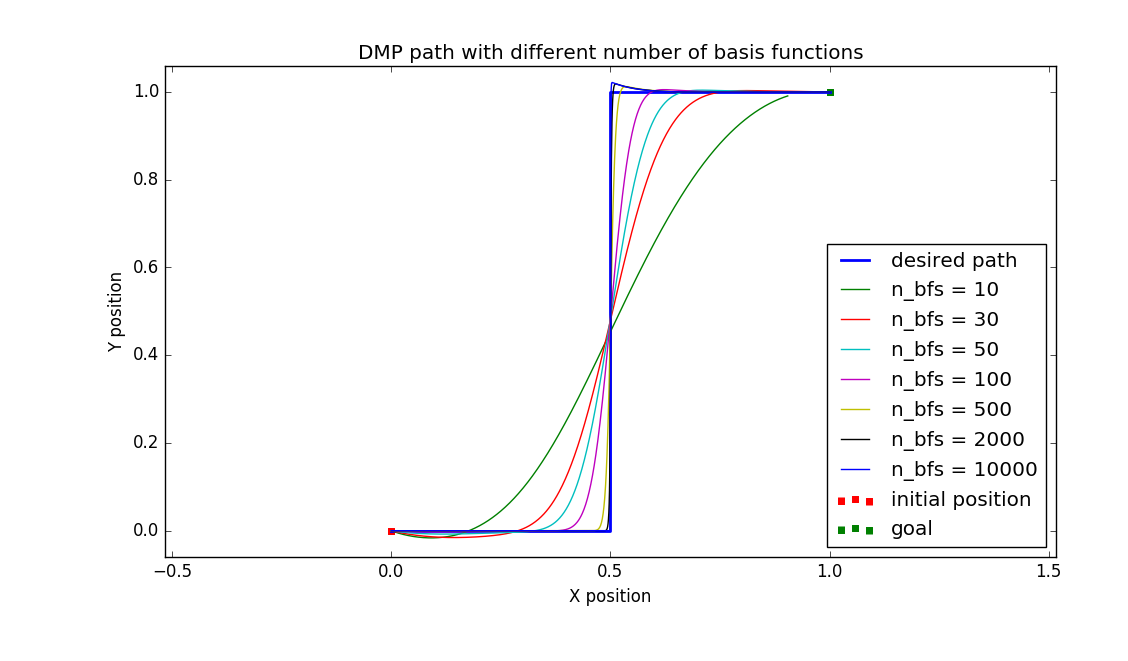
\includegraphics[width=\textwidth]{images/n_bfs_}
	\end{frame}
	
	\begin{frame}
		\centering
		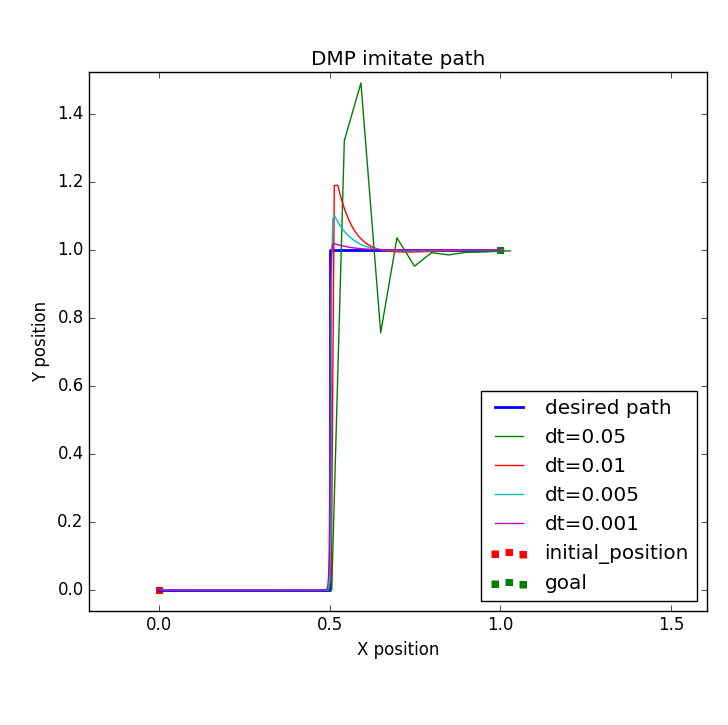
\includegraphics[scale=0.45]{images/dt_}
	\end{frame}
	
	\begin{frame}
		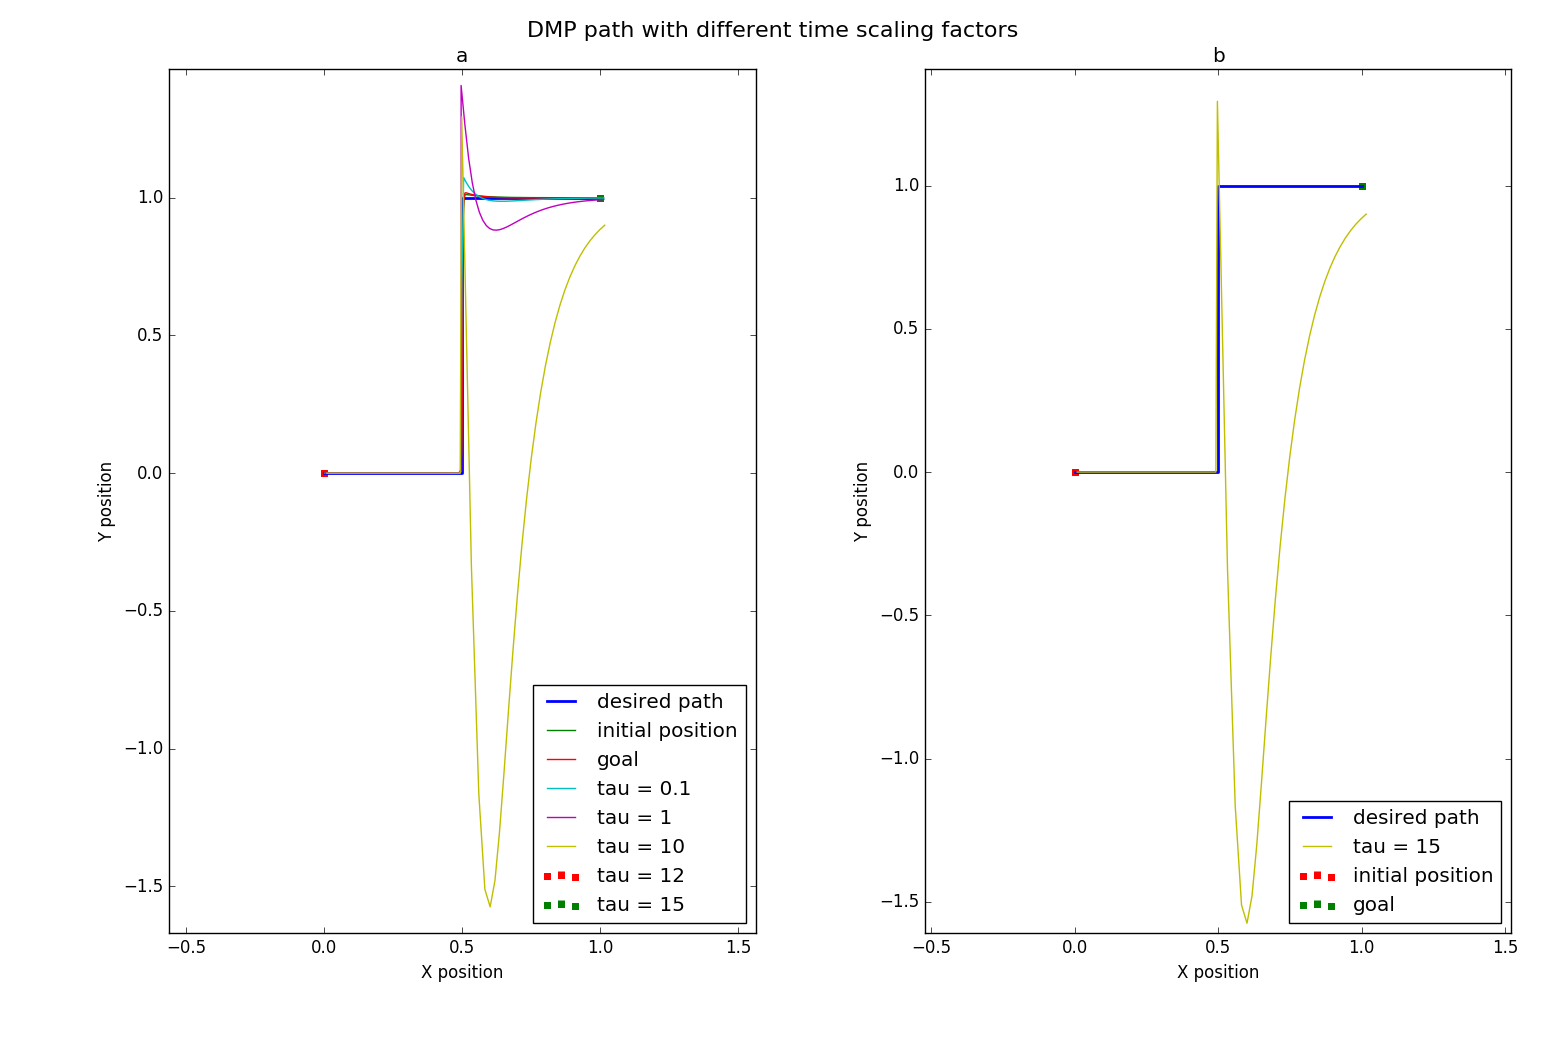
\includegraphics[width=\textwidth]{images/tau_}
	\end{frame}
	
	\begin{frame}{Inverse Kinematic Solver}
		
	\end{frame}
	
	\begin{frame}{Whole Body Motion Control}
		\begin{equation}
		m_{cap} = \frac{(\sigma_{min} - \sigma_{l})}{(\sigma_{h} - \sigma_{l})}
		\end{equation}

		\begin{equation}
		b_{cap} = \frac{(d - d_{l})}{(d_{h} - d_{l})}
		\end{equation}
		
		\begin{equation}
		v_{ee} = m_{cap}.v
		\end{equation} 
		
		\begin{equation}
		v_{b} = (1 - m_{cap}).v
		\end{equation} 

	\end{frame}
	
	\begin{frame}{Experiments}
		\begin{itemize}
			\item 
		\end{itemize}
	\end{frame}
	
	\begin{frame}{Results}
	
	\end{frame}
	
	\begin{frame}{Conclusion}
	
	\end{frame}

\end{document}
